\documentclass{article}


%                          _               
%                         | |              
%    _ __  _   _ _   _ ___| |__  _   _ ___ 
%   | '_ \| | | | | | / __| '_ \| | | / __|
%   | |_) | |_| | |_| \__ \ |_) | |_| \__ \
%   | .__/ \__, |\__,_|___/_.__/ \__,_|___/
%   | |     __/ |                          
%   |_|    |___/                           
%

\usepackage{arxiv}

\usepackage[utf8]{inputenc} % allow utf-8 input
\usepackage[T1]{fontenc}    % use 8-bit T1 fonts
\usepackage{hyperref}       % hyperlinks
\usepackage{url}            % simple URL typesettingf
\usepackage{booktabs}       % professional-quality tables
\usepackage{amsfonts}       % blackboard math symbols
\usepackage{nicefrac}       % compact symbols for 1/2, etc.
\usepackage{microtype}      % microtypography
\usepackage{lipsum}
\usepackage{graphicx}
\usepackage{tabularx}
\usepackage{wrapfig}

\usepackage[export]{adjustbox}

\usepackage{xcolor}         % http://ctan.org/pkg/xcolor

\hypersetup{
  colorlinks=true,
  linkcolor=blue!50!red,
  urlcolor=green!70!black
}

\title{pyusbus: opening usb ultrasound probes}

\author{
  Luc Jonveaux\thanks{More on the website \url{http://un0rick.cc/goodies/usbprobes}. This paper has its on Zenodo DOI  \href{http://doi.org/10.5281/zenodo.5792256}{10.5281/zenodo.5792256} } \\
  Curious, Charleville-Mézières, France\\
  \texttt{pyusbus@un0rick.cc} \\
}

%% Wrapping https://tex.stackexchange.com/questions/55161/how-to-arrange-image-and-text-to-appear-side-by-side

\begin{document}
\maketitle

\begin{abstract}

A number of USB ultrasound probes can be found on the general, open online markets. Bibliography shows that the first probes to be released where mechanical probes, such as the "SeeMore" series by Interson, promising to "turn every computer in your facility into an ultrasound imaging system", providing a "affordable, portable, and easy to use" platform.

Having open drivers and libraries to communicate with ultrasound probes could help of course both probes' users, by supplying an easy to use API, but also researchers, by providing additional insights in the workings of the probes.

Still, the communication with probes is locked by proprietary hardware drivers.  Vendors may open their SDKs, but those could be limited, on several levels. The purpose of this exercise is to show that it is feasible to put together the bases of a common, portable platform to use these c.a. 1000 USD probes.


\emph{ This PDF is also a ZIP that contains the sources files of this PDF and of the code, don't hesitate to have a look. Just rename the file from .PDF to .ZIP and you're ready to go }.
\end{abstract}

\keywords{open-source \and ultrasound \and hardware \and retro-engineering \and usb \and probes  }



%                .-') _  .-') _   _  .-')               
%               ( OO ) )(  OO) ) ( \( -O )              
%    ,-.-') ,--./ ,--,' /     '._ ,------.  .-'),-----. 
%    |  |OO)|   \ |  |\ |'--...__)|   /`. '( OO'  .-.  '
%    |  |  \|    \|  | )'--.  .--'|  /  | |/   |  | |  |
%    |  |(_/|  .     |/    |  |   |  |_.' |\_) |  |\|  |
%   ,|  |_.'|  |\    |     |  |   |  .  '.'  \ |  | |  |
%  (_|  |   |  | \   |     |  |   |  |\  \    `'  '-'  '
%    `--'   `--'  `--'     `--'   `--' '--'     `-----' 


\section{Overview}

Getting signals and images from ultrasound mechanical probes is an interesting step to know what radiofrequency signals mean in ultrasound imaging, be it for non-destructive testing or medical imaging. We have developed two pulse-echo boards \cite{un0rick,lit3rick}, which are achieving this. However, operating them requires extra hardware (electronics, probes, a fair bit of soldering, ..). 

Getting ultrasound images could be more straightforward, especially considering ~1kUSD usb probes available on the market. Their image quality is quite good at first glance.

\subsection{Modus operandi}

We examined the exchanges on the USB ports between the vendor software and the probes, using the excellent Wireshark software. For the sake of operation, the four probes described below were used from within a virtual machine. 

The packets were captured using Wireshark, and parsed using scapy as a pcap-parsing library and pandas for sense-making. A particular attention was paid to the initial packets, preceding the acquisition of first imaging data, identified as the transfer of large packets.

We distinguish between simple commands sent to the probe, which we tried to assemble in patterns, from larger packets which are pages of data sent to the probe for different purposes (beamforming, gain setting, depth, ...). Fig. \ref{fig:Packet307_UP20L} shows the content of a parameters packet supposed to setup the beamforming parameters on the UP20L.

\begin{figure}[htp!]
  \centering
    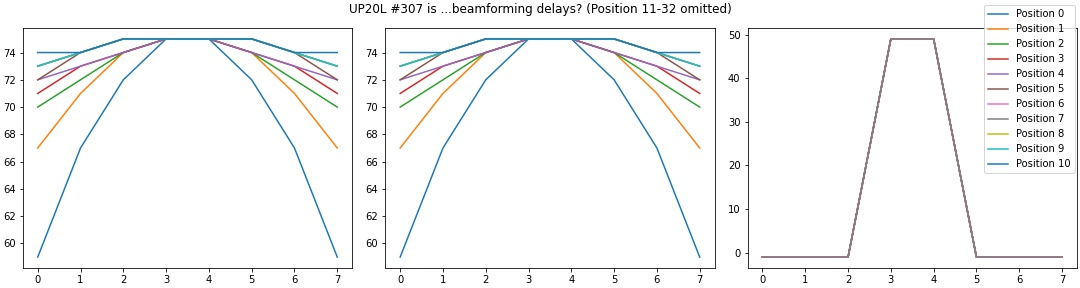
\includegraphics[width=0.98\linewidth]{images/307.jpg}
    \caption{Example of the content of a packet}
    \label{fig:Packet307_UP20L}
  \end{figure}

We logged the different commands sent by software and named them where possible in the subsequent library, \emph{pyusbus}. 

\subsection{Probes}

\subsubsection{Linear, B-mode}

We chose a simple, linar Healson UP20L probe to start the exercise. It appeared to be using from Cypress FX2/FX2LP (USB2) bridge chip, so we used the fx2 python library. The startup pattern was relatively complex, and we tried to simplify it as much as possible.

After a startup, the freeze/unfreeze commands were determined. Images were then obtained.


\subsubsection{Convex, B-mode}

The convex probe was a BMV probe, relatively straightforward to setup.

By default, it exposes images of 80 lines (possibly aligned with a 80-elements probe), each of which has 3900 points per line. This means the "images" are not the enveloppe signals, rather direct radio-frequency, or IQ sampled signals, as seen in Fig. \ref{fig:RF}. 

\begin{figure}[htp!]
  \centering
    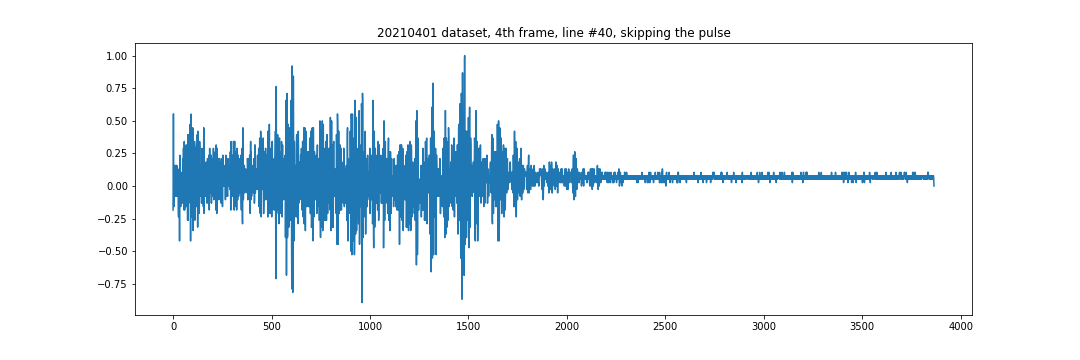
\includegraphics[width=0.98\linewidth]{images/20210401_detail.png}
    \caption{Example of the content of a RF packet}
    \label{fig:RF}
  \end{figure}



\subsubsection{Interson, B-mode}

The Interson is an interesting probe. Older than the rest of the probes, it is based on a different USB2 chip. The device is identified as 0x1921, 0x0001 before being programmed, and 0x1921, 0xf001 after. Interestingly, the family of device was already identified in public repositories \cite{kitware}.

The setup is prepared in two steps, the first ending with a rebook of the probe in a controlable mode. The second is easily verifiable: as the probe is a mechanical one, motor control can be felt and heard.

The major challenge is that as of today, the number of lines per image can vary, as the motor can have slight speed changes. Downstream software postprocessing is needed.

\subsubsection{Linear, Doppler}

This USB3 probe, by default, exposes images of 128 lines for 3584 points per line. Doppler images are arrays of 336 lines of 764 points each. We are not yet clear of the content of the doppler images. We have the option to only get B-mode images or interleaved images, alternating Doppler mode and B-Mode frames. Implementation is still uncertain on the geometry and location of the doppler window.

\section{Challeges}

The major challenge we face is the lack of documentation of the probes, and the time needed to understand how to "cleanly" set them up. One can record all commands sent to set a probe at a given depth, with a given TGC curve, and log everything - but this does not yield a fine view over the controls of the probe. We therefore keep the code open for possible contributors, for newer probes, but also to open finer control over the probes, for example over the beamforming parameters.


\section{Results}

A python class has been developped for each of the above-mentioned probes. It allows a standard acquisition, as well as a freeze/unfreeze control, and leads to allow better TGC controls. Significant work is required to transform this as a full-fledge solution, usable on the market. Figure \ref{fig:images} shows examples of images acquired from the library, or from an OEM software, on a phantom.

\begin{figure}[htp!]
\centering
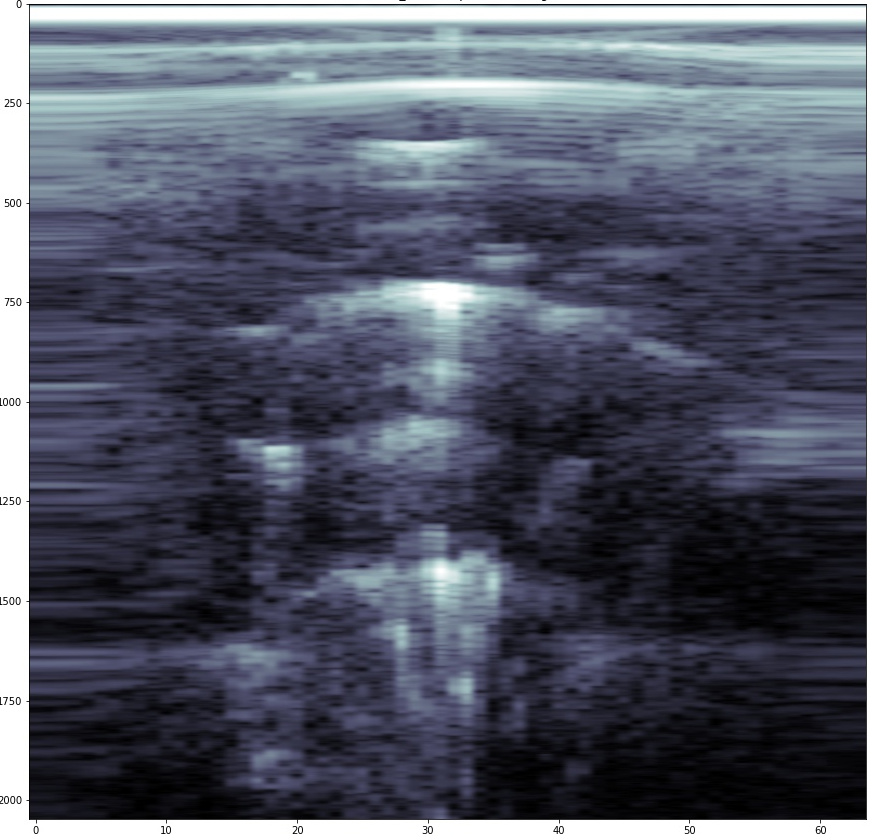
\includegraphics[width=.3\textwidth]{images/interson.jpg}\hfill
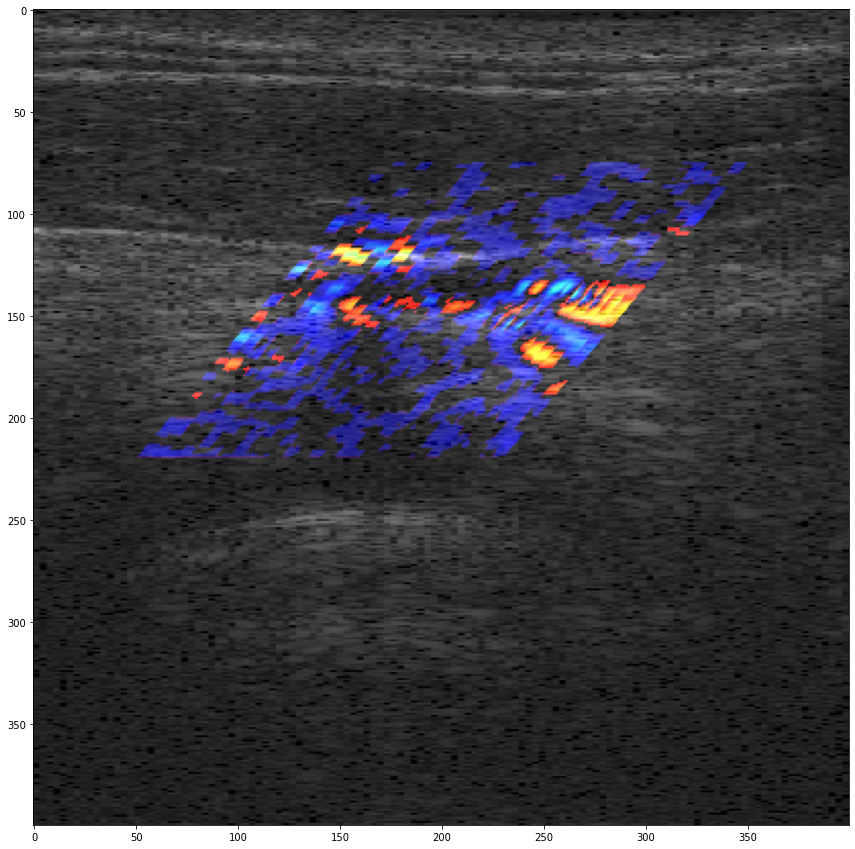
\includegraphics[width=.3\textwidth]{images/doppler_overlay_threshold.png}\hfill
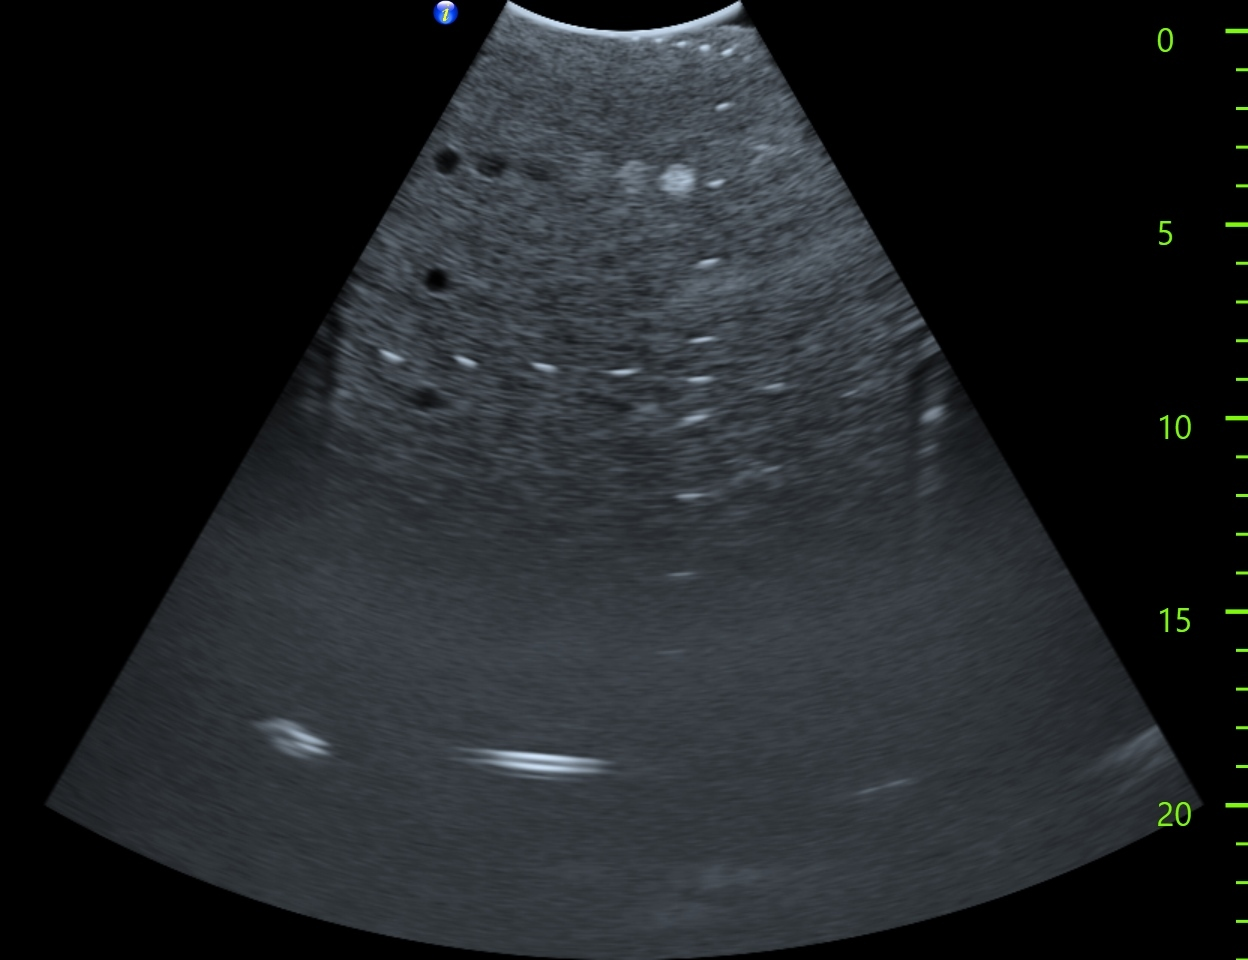
\includegraphics[width=.3\textwidth]{images/202103190001_0001_009.jpg} 
\caption{Example of images using the interson, doppler and convex probes.} 
\label{fig:images}
\end{figure}
 

\section{Next steps}

We hope that delivering this library would open a window of opportunity for current ultrasound researcher.

The note showed the state of the library, at the end of 2021. Four devices were examined and made accessible through its API. It has shown a variety of devices, which surprisingly may have more options accessible for researchers, and not exposed by the manufacturers - for example exposition of raw signals, and not image enveloppes, or access to configuration registers not thought accessible.

This can be promising to allow working on affordable development platforms.

Plenty to do on the next steps! The current shopping list (non-exhaustive) may include:

\begin{itemize}
\item Improving the documentation in general.
\item Work with other probes.
\item Explore remaining controls on current devices. 
\item Keep pcaps for each probe on given settings - pcaps without any large data transfers.
\item Onboard your contribution to open the world of ultrasound imaging!
\end{itemize}

Feel free to use and cite this work!


%    _     _ _     _ _       
%   | |   (_) |   | (_)      
%   | |__  _| |__ | |_  ___  
%   | '_ \| | '_ \| | |/ _ \ 
%   | |_) | | |_) | | | (_) |
%   |_.__/|_|_.__/|_|_|\___/ 
%                        
                         
\bibliographystyle{unsrt}  
\begin{thebibliography}{1}

\bibitem{kelu124}
Luc Jonveaux 2017.
\newblock  Arduino-like development kit for single-element ultrasound imaging. 
\newblock In {\em  Journal of Open Hardware, 1(1), p.3}. DOI: \href{http://doi.org/10.5334/joh.2}{10.5334/joh.2}

\bibitem{pyusb}
Luc Jonveaux 2018.
\newblock The pyusbus repository.
\newblock Website at {\em\href{https://github.com/kelu124/pyusbus}{https://github.com/kelu124/pyusbus}}

\bibitem{kitware}
Matthieu Heitz 2014.
\newblock Interson Manager.
\newblock Website at {\em\href{https://github.com/KitwareMedical/IntersonManager}{https://github.com/KitwareMedical/IntersonManager}}

\bibitem{un0rick}
Luc Jonveaux 2019.
\newblock  un0rick : open-source fpga board for single element ultrasound imaging
\newblock On {\em  Zenodo}. DOI: \href{http://doi.org/10.5281/zenodo.3364559}{10.5281/zenodo.3364559}

\bibitem{lit3rick}
Luc Jonveaux 2021.
\newblock lit3rick: an up5k ultrasound pulse-echo device %%@todo change title
\newblock On {\em  Zenodo}. DOI: \href{http://doi.org/10.5281/zenodo.5792245}{10.5281/zenodo.5792245}

\bibitem{mux}
Luc Jonveaux 2021.
\newblock An open-source max14866 development board %%@todo change title
\newblock On {\em  Zenodo}. DOI: \href{http://doi.org/10.5281/zenodo.5792252}{10.5281/zenodo.5792252}

\bibitem{probes}
Luc Jonveaux 2021.
\newblock  pyubus: opening usb ultrasound probes  %%@todo change title
\newblock On {\em  Zenodo}. DOI: \href{http://doi.org/10.5281/zenodo.5792256}{10.5281/zenodo.5792256}

\end{thebibliography}

\end{document}


